\subsection{SnakeManager}
\label{section:SnakeManager}

The SnakeManager has the responsibility for handling all game logic having to do with the snake. Its primary areas of concern are: Initializing and updating an array representing the snake, adding a new body part to the snake when it hits a piece of food, and detecting whether or not the snake collides with itself.

Figure \ref{SnakeManagerClassDiagram} shows a class diagram of the SnakeManager.

\begin{figure}[H]
	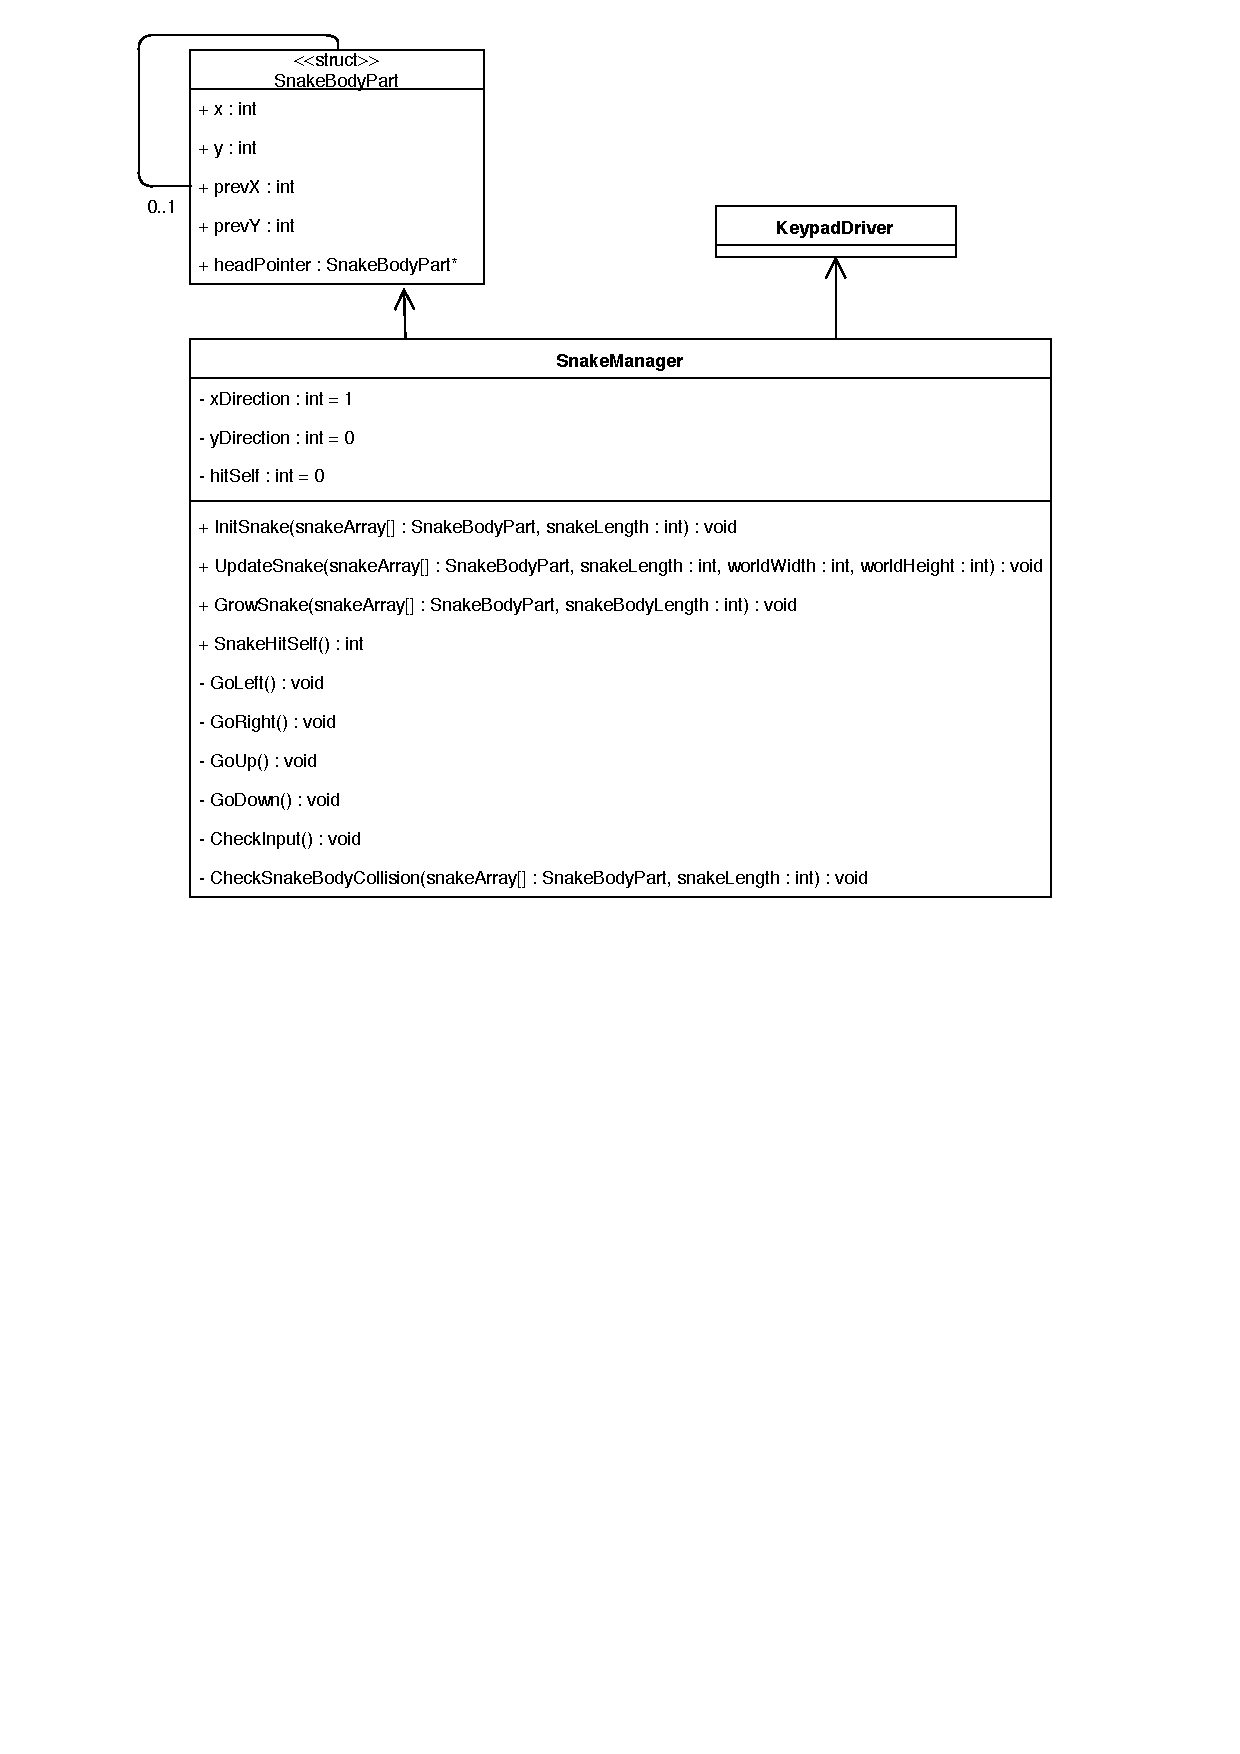
\includegraphics[scale=0.75]{SnakeManagerClassDiagram}
	\centering
	\caption{Class diagram for SnakeManager}
	\label{SnakeManagerClassDiagram}
\end{figure} 

As can be seen in figure \ref{SnakeManagerClassDiagram}, The SnakeManager makes use of the KeypadDriver. This driver is described in section \ref{section:MatrixKeyboard} - \nameref{section:MatrixKeyboard}.

Also, the SnakeManager makes use of a struct by the name of SnakeBodyPart. This struct represents a single part of the snake's body. It is by these body parts that the snake grows - one by one. 

Table \ref{table:SnakeBodyPartAttributeDescriptions} contains descriptions of the attributes of the SnakeBodyPart struct.

\begin{table}[H]
	\centering
	\begin{tabular}{|l|l|}
		\hline
		Attribute & Description \\ \hline
		x & The X position of the body part in world space. \\ \hline
		y & The Y position of the body part in world space. \\ \hline
		prevX & \begin{tabular}[c]{@{}l@{}}The X position of the body part in the\\ previous frame of the game loop.\end{tabular} \\ \hline
		prevY & \begin{tabular}[c]{@{}l@{}}The Y position of the body part in the previous\\ frame of the game loop.\end{tabular} \\ \hline
		headPointer & \begin{tabular}[c]{@{}l@{}}A pointer to the SnakeBodyPart which this\\ SnakeBodyPart is chained to.\end{tabular} \\ \hline
	\end{tabular}
	\caption{Descriptions of the attributes for the SnakeBodyPart struct, used by the SnakeManager}
	\label{table:SnakeBodyPartAttributeDescriptions}
\end{table} 

Table \ref{table:SnakeManagerAttributeDescriptions} contains descriptions for the attributes of SnakeManager.

\begin{table}[H]
	\centering
	\begin{tabular}{|l|l|}
		\hline
		Attribute & Description \\ \hline
		xDirection & \begin{tabular}[c]{@{}l@{}}The current direction of the snake along the\\ x-axis of the display.\\ \\ 1 = Right\\ -1 = Left\\ 0 = No horizontal direction\end{tabular} \\ \hline
		yDirection & \begin{tabular}[c]{@{}l@{}}The current direction of the snake along the\\ y-axis of the display.\\ \\ 1 = Down\\ -1 = Up\\ 0 = No vertical direction\end{tabular} \\ \hline
		hitSelf & \begin{tabular}[c]{@{}l@{}}An indication of the snake hitting itself.\\ \\ 1 = The snake collided with itself\\ 0 = The snake did not collide with itself\end{tabular} \\ \hline
	\end{tabular}
	\caption{Descriptions for the SnakeManager attributes}
	\label{table:SnakeManagerAttributeDescriptions}
\end{table}

Table \ref{table:SnakeManagerMethodDescriptions} contains descriptions of highlighted methods of the SnakeManager.

\begin{table}[H]
	\centering
	\begin{tabular}{|c|c|}
		\hline
		\textbf{Method} & \textbf{Description} \\ \hline
		InitSnake & \begin{tabular}[c]{@{}c@{}}This method accepts an array from a client (snakeArray)\\ which should be used to construct a snake with a length\\ of SnakeBodyParts specified by the snakeLength parameter.\end{tabular} \\ \hline
		UpdateSnake & \begin{tabular}[c]{@{}c@{}}This method will move the snake each frame of the game loop. \\ The parameters worldWidth and worldHeight is used\\ by the method to calculate world bounds.If the snake exceeds\\ these bounds, it will reappear on the opposite side of where\\ it exited.\end{tabular} \\ \hline
		GrowSnake & \begin{tabular}[c]{@{}c@{}}This method will grow the snake to a new size. It is used\\ when the snake picks up a piece of food.\end{tabular} \\ \hline
		SnakeHitSelf & \begin{tabular}[c]{@{}c@{}}This will is used by clients to figure out if the snake has\\ hit itself. A return value of 1 indicates collision, and a value of\\ 0 indicates no collision.\end{tabular} \\ \hline
		CheckSnakeBodyCollision & \begin{tabular}[c]{@{}c@{}}This method performs collision detection to see if the\\ snake has hit itself.\end{tabular} \\ \hline
	\end{tabular}
	\caption{Descriptions of highlighted methods of the SnakeManager}
	\label{table:SnakeManagerMethodDescriptions}
\end{table}

\subsubsection{Snake Management}
The way that the snake is represented and managed through the game is by an array of the aforementioned SnakeBodyPart structs. Figure \ref{SnakeBodyPartManagement} illustrates this.

\begin{figure}[H]
	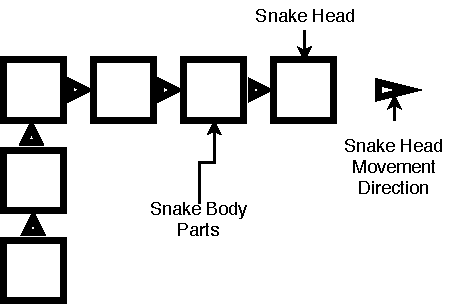
\includegraphics[scale=1.0]{SnakeBodyPartManagement}
	\centering
	\caption{Illustration of the snake being made up of a chain of SnakeBodyParts}
	\label{SnakeBodyPartManagement}
\end{figure} 

Essentially, the snake is a singly linked list \cite{LinkedLists} of SnakeBodyParts. Each SnakeBodyPart, as described in table \ref{table:SnakeBodyPartAttributeDescriptions}, has a pointer to a SnakeBodyPart that comes next in the chain. it's a recursive struct.

Every time the game advances a single frame, the head of the snake moves a certain amount of world units in a direction determined by the user. Afterwards, each chained SnakeBodyPart advances themselves to the previous position of its chained SnakeBodyPart. This makes all parts of the snake move as a coherent whole. This update process is illustrated in figure \ref{SnakeBodyPartUpdateProcess}.

\begin{figure}[H]
	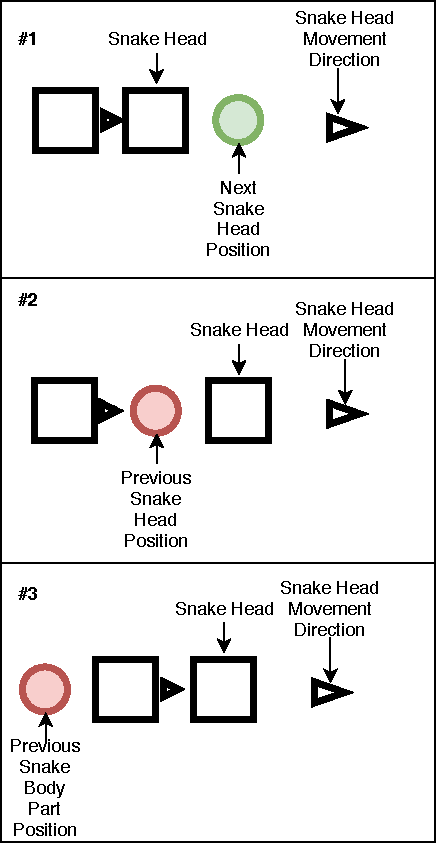
\includegraphics[scale=0.75]{BodyPartsUpdatingIllustration}
	\centering
	\caption{Illustration of the SnakeBodyPart update process}
	\label{SnakeBodyPartUpdateProcess}
\end{figure} 

\subsubsection{Collision Detection}
\label{section:CollisionDetection}

Collision detection on the snake is handled by use of Axis-Aligned Bounding Box Collision Detection \cite{CollisionDetection}. Essentially, this type of collision detection checks if two rectangles (aligned by axes, no rotation applied) overlap. If they overlap, a collision is reported. The advantage of this type of collision detection algorithm is that it is relatively simple to implement and it is fast to execute - which fits well when the game executes on a microcontroller with limited CPU resources. Since our game makes use of simple box shapes for the snake body parts, this algorithm fits very well with this type of game.







